\chapter{Yara}
\label{sec:yara}

\emph{Yara} (\emph{Y}et \emph{a}nother \emph{r}ead \emph{a}ligner) is an exhaustive, non-heuristic read mapper, capable of quickly reporting all stratified mapping locations within a given error rate.
Yara works with Illumina or Ion Torrent reads, supports both paired-end and mate-pair protocols, computes accurate mapping qualities, offers parallelization via multi-threading, has a low memory footprint thanks to the FM-index, and does not require ad-hoc parameterization.

% -----------------------------------------------------------------------------

\section{Engineering}
\label{sec:yara:eng}

\subsection{Stratified mapping}
\label{sec:yara:eng:strata}

Yara follows the concept of stratified all-mapping.
The all-mapping methods discussed so far consider a set of relevant mapping locations per read.
Yet, this definition leaves open what relevant means.
In all-mapping under the edit distance, the user defines relevant mapping locations by imposing a distance threshold.
Despite being sound, this definition does not work well in practice.
On the one hand a very low threshold leaves a consistent fraction of the reads unmapped, on the other hand a moderate threshold produces a deluge of mapping locations for some reads.
In practice, at 5\,\%, error rate, Illumina reads map on average to hundreds of mapping locations on the human genome.
It is questionable whether all these locations are relevant for the downstream analysis.
Thus, a finer definition of all-mapping relevance is necessary in practice.

%\subsubsection{Stratified mapping}

Stratification of mapping locations yields an equally sound yet practical definition of all-mapping under the edit distance.
The $e$-stratum
\begin{eqnarray}
S_e = \{ (i,j,e) : d_E(g_{i \dots j},r) = e\}
\end{eqnarray}
denotes the set of all mapping locations of a read $r$ at edit distance $e$ from the reference genome $g$.
According to the above definition, conventional all-mapping under the edit distance defines the set
\begin{eqnarray}
S^* = S_0 \cup S_1 \cup \dots \cup S_k
\end{eqnarray}
as relevant mapping locations within an \emph{absolute} error threshold $k$.
Stratified all-mapping refines this definition by considering only mapping locations being co-optimal, or sub-optimal up to a certain degree.
Formally, if the distance of any optimal mapping location for read $r$ is
\begin{eqnarray}
e^* = \min \,\{ e \in [0,k] : S_e \neq \emptyset \}
\end{eqnarray}
stratified all-mapping considers mapping locations
\begin{eqnarray}
S^l = S_{e^*} \cup \dots \cup S_{\min \,\{ e^*+l, k\}}
\end{eqnarray}
within a \emph{relative} error threshold $l$ to be relevant.
%Note that $l \ll k$.

\subsubsection{Efficient filtration by strata}

Yara significantly improves the runtime of stratified all-mapping over conventional all-mapping.
Obviously, the most straightforward way to achieve stratified all-mapping consists into performing conventional all-mapping and subsequently filtering out any irrelevant mapping location.
For instance, RazerS\,3 implements this method and gets no speedup.
Another na\"ive method consists into applying up to $k$ rounds of conventional all-mapping, using filtration schemes for thresholds going from $0$ to $\min \,\{ e^*+l, k\}$.
It is easy to see that also this method performs redundant computation: the total work for any read that maps at distance greater or equal to $k$ corresponds to the sum of all $k$ filtration schemes.

The following stratified all-mapping method, implemented in Yara, guarantees not to perform more work than conventional all-mapping.
Indeed, the key idea is to simply reduce any filtration scheme full-sensitive within distance $k$ to be full-sensitive within distance $\min \,\{ e^*+l, k\}$.
Given a filtration scheme $\mathbf{t}=(t_1,\dots,t_s)$ full-sensitive within distance $k$, any subset consisting of $s^* \leq s$ seeds with thresholds $\mathbf{t^*}=(t^{*}_{1},\dots,t^{*}_{s^*})$ is full-sensitive within distance $\min \,\{ e^*+l, k\}$ if it satisfies
\begin{eqnarray}
s^* + \sum_{i=1}^{s^*} t_i^* > \min \,\{ e^*+l, k\}.
\end{eqnarray}
%The proof is analogous to that one given in section~\ref{sec:seeds-apx}.
%Verification of all candidate locations produced by one seed or by one threshold accounts for one stratum $S(r,i)$.

\begin{example}
Let $k=5$ be the absolute threshold, and $l=0$ be the relative threshold, restricting relevant locations to co-optimal ones.
A read $r$ maps at distance 1, \ie $|S(r,0)| = 0$ and $|S(r,1)| > 0$, thus $e^* = 1$.
Given the filtration scheme $\mathbf{t}=(1,1,1)$, any subset full-sensitive up to distance $\min \,\{ e^*+l, k\} = 1$ finds all relevant mapping locations.
All full-sensitive subsets of $\mathbf{t}$ are $(0,0,-)$, $(0,-,0)$, $(-,0,0)$, $(1,-,-)$, $(-,1,-)$, $(-,-,1)$, where a $-$ at position $i$ indicates that the $i$-th seed is unnecessary.
Thus, the verification of all candidates, either produced by \emph{any} two exact seeds or by one 1-approximate seed, yields all mapping locations in the $1$-stratum of $r$.
\end{example}

\subsubsection{Greedy verification strategy}

In addition, Yara implements a simple greedy strategy to minimize the number of verifications necessary to find all relevant stratified mapping locations.
As candidate locations can be verified in any order, Yara chooses an ordering of seeds producing the minimum number of verifications.
The tool first finds all seeds and ranks them by number of candidate locations produced.
Then it processes all candidate locations, from the least to the most frequent seed, until it explores $l$ strata from the first non-empty one, or until it attains the absolute distance threshold $k$.

Yara performs best-mapping by means of stratified filtration.
Best-mapping requires one primary mapping location along with its confidence.
Under the edit distance, without any further assumptions, any co-optimal location is equally likely to be correct.
Thus, Yara performs stratified all-mapping with a relative threshold $l=0$, picks one random co-optimal location, and subsequently estimates its mapping quality using all found mapping locations (see section~\ref{sec:yara:eng:qualities}).
Thanks to this method, Yara in best-mapping is an order of magnitude faster than in all-mapping.

%Yara uses mapping strata to compute precise mapping qualities and to perform paired-end mapping.

\subsection{Adaptive filtration}
\label{sec:yara:eng:adaptive}

Specific yet rapid filtration is fundamental in the design of an efficient read mapping tool.
Read mappers like RazerS\,3 \citep{Weese2012} and mrFast \citep{Ahmadi2012} are designed around na\"ive filtration with exact seeds.
This filtration method is always very quick, however it is not specific enough on long, repetitive reference genomes like the human genome.
Masai \citep{Siragusa2013} circumvents this problem by enforcing a minimum seed length,
whose optimal value must be tuned for a specific reference genome, and eventually resorting to approximate seeds in order to guarantee full-sensitivity.
This filtration method speeds up Masai by an order of magnitude but has some drawbacks:
it needs external parametrization, lacks flexibility and is suboptimal in practice.

Yara applies an adaptive filtration scheme \emph{per read} because, under any fixed filtration scheme, the number of verifications per read is not uniform: within a typical human genome resequencing, most reads produce very few verifications and are easily mappable, while few other reads are problematic and often not even confidently mappable to one single location.
Consequently, any fixed filtration scheme turns out to be too weak for some reads yet too strong for others, thus suboptimal in practice.
An adaptive filtration scheme per read improves filtration efficiency by optimizing the ratio between filtration speed and specificity.
Yara thus automatically chooses an adaptive filtration scheme per read, without requiring manual parameterization by the user.

Adaptive filtration works as follows.
Yara initially applies filtration with exact seeds to all reads.
The tool counts the number of verifications to be performed for each read, thus decides if it is worth proceeding with the verification phase or alternatively applying a stronger filtration scheme.
This decision depends on fine-tuned internal verification thresholds.
Under standard Illumina setups, exact seeds provide efficient filtration for up to 70--80\,\% of the reads; on the remaining reads, a filtration scheme using $1$-- or $2$--approximate seeds works better.
Thus, Yara starts with the quickest filtration scheme and becomes more specific whenever it pays off to do so.

%For instance, when mapping 100\,bp Illumina reads on the human genome within 5\,\% error rate, filtration with exact seeds produces 6 exact seeds of length 16\,bp;
%under these terms, a single read produces an average of 15000 verifications, and the verification phase takes 99\,\% of the runtime.
%On the same mapping setup, this method produces 3 $1$--approximate seeds of length 33\,bp; thus a single read produces 1400 verifications on average.
%Under this setup, Masai in all-mapping still spends about 20\,\% of its runtime in filtration and the remaining 80\,\% in verification.
%The next stronger filter produces 2 $2$--approximate seeds of length 50\,bp.

\subsection{Indexing}
\label{sec:yara:eng:indexing}

Yara uses an efficient FM-index specialization for the DNA alphabet, based on interleaved rank dictionaries (see section~\ref{sec:index:succinct:rd}).
This interleaved FM-index exhibits a fourfold speedup over the first FM-index implementation bundled with Masai.
Surprisingly, the interleaved FM-index is also faster than any other index, both in exact and approximate search (see section~\ref{sec:index:algo}).
Moreover, this index consumes only 1.23 bytes per base pair with a SA sampled at 10\,\%, thus its memory footprint for the human genome is 3.7~GB.
Under these terms, there is no space-time indexing trade-off: the FM-index always provides the most convenient suffix trie implementation.

Yara does not use the multiple search algorithms of section~\ref{sec:index:algo:multimismatch} to search seeds on the FM-index.
As shown in section~\ref{sec:index:algo}, on the FM-index it is always faster to search exact queries in a na\"ive way and approximate queries after sorting them in lexicographical order.
This fact considerably simplifies a fine-grained parallelization of the tool.

%Yara implements fine-grained parallelism.
%It would be possible to stream over reads to parallelize computation per read.
%However, the tool processes batches of reads.


\subsection{Paired-end and mate-pair protocols}
\label{sec:yara:eng:pairs}
Paired-end and mate-pair protocols are the sequencing protocols of choice of Illumina instruments.
Reads are sequenced in pairs from both ends of the same insert.
Properly paired reads are expected to map within the insert size adopted in the sequencing protocol.
Thus, the added information of an expected insert size allows a read mapper to map read pairs to their original locations more confidently than in the single-end protocol.
Nonetheless, a read mapper should report equally important unpaired mapping locations, as the lack of any proper pair of mapping locations signals a potential structural variation, \eg a long indel or an inversion.

In the paired-end or mate-pair workflows, Yara maps paired reads independently, exactly as in the single-end workflow, and reports all relevant mapping locations per read.
However, in addition to the single-end workflow, Yara implements a finer strategy to choose primary mapping locations.
For any reads pair, among all pairs of co-optimal mapping locations, the tool selects the one with minimal deviation from the expected insert size.
Since Yara outputs all relevant mapping locations, the choice of primary locations can be always corrected a posteriori.

\subsection{Mapping qualities}
\label{sec:yara:eng:qualities}
Yara computes accurate mapping qualities using the number of found mapping locations stratified by error rate.
In section~\ref{sec:yara:eng:strata} I defined the set $S$ of all relevant mapping locations as
\begin{eqnarray}
S = \bigcup_{e=0}^{k} S_e.
\end{eqnarray}
I now denote by $z_e$ the number of mapping locations in the stratum $S_e$, \ie $z_e=|S_e|$;
I associate to $S$ a canonical partition function $Z$
\begin{eqnarray}
\label{eq:yara:mqual:partition}
Z = \sum_{e=0}^{k} z_e w(e),
\end{eqnarray}
where the function $w : \N \rightarrow \R$ assigns a weight to each (sub)optimal stratum.

\subsubsection{Single-end reads}

For a fixed single-end read, I denote with $C$ a random variable assuming the value of its correct mapping location, and I assume that
\begin{eqnarray}
\Pr[C \in S] = 1.
\end{eqnarray}
I estimate the probability of $C$ being part of the stratum $S_e$ as
\begin{eqnarray}
\label{eq:yara:mqual:se:stratum}
\Pr[C \in S_e] = \frac{1}{Z} \cdot z_e w(e)
\end{eqnarray}
and the probability of $C$ being equal to any found mapping location $(i,j,e)$ as
\begin{eqnarray}
\label{eq:yara:mqual:se:location}
\Pr[C = (i,j,e)] = \frac{1}{Z} \cdot w(e).
\end{eqnarray}

%In practice, I define $w$ as:
%\begin{eqnarray}
%w(e) = ...
%\end{eqnarray}

Hence, equation~\ref{eq:yara:mqual:se:location} gives the probability $p$ that a random mapping location drawn from any stratum is correct.
Such probability $p$ is further encoded as the mapping quality $Q=-10 \log_{10}(1-p)$.

\subsubsection{Paired-end reads}

A paired-end read whose mate is unmapped is treated as a single-end read, thus the above probabilities still hold.
Given a read end, I denote by $S'_e$ the $e$-stratum of its mate, by $Z'$ the canonical partition function of its mate as in equation~\ref{eq:yara:mqual:partition}, and by $C'$ its correct mapping location.
I partition each stratum $S_e$ in two subsets $S^P_e$ and $S^I_e$, where $S^P_e$ contains all mapping locations in $S_e$ being properly paired to some mapping location in $S'$, and $S^I_e = S^P_e \setminus S_e$.
I distinguish the cases of a read end having some properly paired mapping location or not.

If a read end has no properly paired mapping location, $S^I_e = S_e$.
I estimate the probability of $C$ being equal to any found mapping location $(i,j,e)$ as
\begin{eqnarray}
\Pr[C = (i,j,e) | S^P_e = \emptyset] = \Pr[C = (i,j,e)] \cdot \Pr[C' \not{\in} S'_{e'}]
\end{eqnarray}
and since
\begin{eqnarray}
\Pr[C' \not{\in} S'_{e'}] = 1 - \frac{1}{Z'} \cdot z_{e'} w(e'),
\end{eqnarray}
it follows that
\begin{eqnarray}
\label{eq:yara:mqual:pe:location}
\Pr[C = (i,j,e) | S^P_e = \emptyset] = \frac{1}{Z} \cdot w(e) - \frac{1}{ZZ'} \cdot z_{e'} w(e) w(e').
\end{eqnarray}

Now I consider the case of a read end having some properly paired mapping location.
In this case, Yara picks a random location from $S^P_e$, under the assumption that any location in $S^P_e$ is more likely to be correct than those in $S^I_e$.
Therefore, I assign different weights to $S^P_e$ and $S^I_e$.
I assume that
\begin{eqnarray}
\Pr[C \in S^P] = \Pr[C' \in S^{P'}_{e'}] = p'
\end{eqnarray}
and 
\begin{eqnarray}
\Pr[C \in S^I] = 1 - p'.
\end{eqnarray}
Hence the probability of $C$ being part of the properly paired locations in stratum $S_e$ is
\begin{eqnarray}
\label{eq:yara:mqual:se:stratum}
\Pr[C \in S^P_e] = \frac{p' z^p_e w(e)}{p' * Z^P + (1-p') * Z^I}
\end{eqnarray}
and the probability that any of these locations is correct as
\begin{eqnarray}
\label{eq:yara:mqual:se:location}
\Pr[C = (i,j,e) \in S^P_e] = \frac{p' w(e)}{p' * Z^P + (1-p') * Z^I}.
\end{eqnarray}


% -----------------------------------------------------------------------------

\section{Evaluation}
\label{sec:yara:eval}

The evaluation consists of three experiments, all performed on the human reference genome (GRCh37).
The first experiment assesses all-mapping sensitivity by applying the Rabema benchmark on real data.
The second experiment evaluates best-mapping accuracy on simulated data.
The last experiment assesses the performance of best-mappers within a variant calling pipeline applied to real data.

All experiments consider also read mapping throughputs and memory consumptions.
Read mapping throughput is measured in \emph{giga base pairs per hour} (Gbp/h).
The Illumina HiSeq\,2500 in a six days run produces\footnote{According to the specifications at \url{http://res.illumina.com/documents/products/datasheets/datasheet_hiseq2500.pdf} for high output run mode with dual flow cell.} up to 800~Gbp as $2 \times 100\,\text{bp}$ paired-end reads.
Under this measure the maximum throughput of the Illumina HiSeq\,2500 is $5.56$ Gbp/h.
%Runtimes for each tool are measured on de-facto standard input and output formats, \ie they consider the time to produce a compressed BAM file from a gzipped FastQ file.

In addition to Yara, I consider the following state-of-the-art tools: Bowtie\,2, BWA, GEM, RazerS\,3, and Hobbes\,2.
Bowtie\,2 and BWA are suited for best-mapping, while RazerS\,3 and Hobbes\,2 for all-mapping.
GEM, in addition to all-mapping, can be used for best-mapping only to some extent, as it does not compute mapping qualities.

\subsection{Experimental setup}

\subsubsection{Read mappers parametrization}

In appendix \ref{sup:yara:param}, I give the exact parametrization of each read mapper considered in the evaluation.
Whenever possible, I configured the tools with the appropriate error rate (Yara, GEM, RazerS\,3) or absolute number of errors (Hobbes\,2).
When processing paired-end reads, I provided the tools with appropriate insert size information.

\subsubsection{Infrastructure}

All tools run on a desktop computer running Linux~3.10.11, equipped with one Intel\textsuperscript{\textregistered} Core i7-4770K CPU @ 3.50\,GHz, 32\,GB RAM and a 2\,TB HDD @ 7200\,RPM.
For maximum throughput, all tools run using eight threads.
For accurate running time comparisons, I disabled Intel Turbo Boost; therefore, all measured running times might be slightly higher than the actual ones.

\subsection{Rabema benchmark on real data}
\label{sec:yara:eval:rabema}

The first experiment uses the Rabema benchmark to evaluate all-mappers sensitivity on real data.
The \emph{Rabema benchmark} \citep{Holtgrewe2011} (v1.2) measures the sensitivity of read mappers in finding \emph{relevant} mapping locations of genomic reads.
This experiment is subdivided in two categories: \emph{suboptimal} and \emph{co-optimal}.
In the category suboptimal, Rabema counts as relevant, for each read, all suboptimal mapping locations within a maximal edit distance error rate, \ie all strata; in the category all-best it considers just co-optimal mapping locations, \ie only the best stratum.
Rabema computes the \emph{sensitivity} of each tool as the fraction of relevant mapping locations found per read.
For a thorough evaluation, Rabema classes mapping locations by their \emph{error rate}, then computes sensitivity within each error rate class.
The benchmark reports percentual scores normalized by the number of reads.

The data used in this experiment is a publicly released sequencing run (SRA/ENA id: ERR161544) by the Beijing Genome Institute;
the genomic DNA used in this study came from an anonymous male Han Chinese individual who has no known genetic diseases.
This dataset consists of $2 \times 100\,\text{bp}$ whole genome sequencing reads produced by an Illumina HiSeq 2000 instrument.
For practical reasons, in the category \emph{co-optimal} I consider the first $10\,\text{M}$ reads, while in the category \emph{suboptimal} only the first $1\,\text{M}$ reads.

An error rate of 5\,\%, is sufficient to map almost all reads in the dataset.
Therefore, I built a Rabema gold standard by running RazerS\,3 in full-sensitive mode within 5\,\% error rate.
Subsequently, I provided the reads as unpaired to each tool, as the Rabema benchmark is not meaningful for paired-end reads.

\begin{table*}[t]
  \caption[Yara results in the Rabema benchmark]
  {
  \label{tab:yara:rabema}
    Rabema benchmark results.
    The left panel shows the results of finding all co-optimal mapping locations of $10\,\text{M}$ whole human genome $100\,\text{bp}$ Illumina HiSeq 2000 reads; the right panel shows the results of finding all suboptimal mapping locations of only the first $1\,\text{M}$ reads.
    Big numbers show total Rabema scores, while small numbers show marginal scores for the mapping locations at
    $\bigl(\begin{smallmatrix}\mbox{\tiny 0}&\mbox{\tiny 1}&\mbox{\tiny 2}\\\mbox{\tiny 3}&\mbox{\tiny 4}&\mbox{\tiny 5}\end{smallmatrix}\bigr)$ \% error rate.
    }
  \vspace{-3mm}
  \center
  \sffamily
  \resizebox{0.95\textwidth}{!}
  {
	\renewcommand{\tabcolsep}{0.8ex}
	% latex table generated in R 2.15.0 by xtable 1.7-0 package
% Sun Apr 19 16:03:47 2015
\begin{tabular}{lcrr}
  \toprule
   
    &\multicolumn{1}{c}{  Co-opt. locations } &\multicolumn{1}{r}{  Throughput } &\multicolumn{1}{r}{  Memory } \\
   &\multicolumn{1}{c}{ \footnotesize [\%] } &\multicolumn{1}{r}{ \footnotesize [Gbp/h] } &\multicolumn{1}{r}{ \footnotesize [GB] } \\
  \midrule
 Yara [s=0]  & \cellcolor[rgb]{0.40425617820036,0.713704577097772,0.548968486936165}\phantom{}100.0 {\subcolbeg\begin{tabular}{rrr} \cellcolor[rgb]{0.403921568627451,0.713725490196078,0.549019607843137}\phantom{}100.0 & \cellcolor[rgb]{0.403921568627451,0.713725490196078,0.549019607843137}\phantom{}100.0 & \cellcolor[rgb]{0.404100695885258,0.713714294742466,0.54899224117875}\phantom{}100.0\\ \cellcolor[rgb]{0.404911039359379,0.713663648275333,0.548868438703537}\phantom{}100.0 & \cellcolor[rgb]{0.411736967340121,0.713237027776537,0.547825588595368}\phantom{0}99.8 & \cellcolor[rgb]{0.43280413151621,0.711920330015531,0.544606994068466}\phantom{0}99.4\subcolvspace\\\end{tabular}\subcolend} & 13.59\ \  & 4.88 \\ 
   GEM  & \cellcolor[rgb]{0.406658255369263,0.713554447274715,0.548601502924249}\phantom{0}99.9 {\subcolbeg\begin{tabular}{rrr} \cellcolor[rgb]{0.403926957971223,0.713725153362093,0.549018784471172}\phantom{}100.0 & \cellcolor[rgb]{0.404751642606762,0.713673610572372,0.548892790985187}\phantom{}100.0 & \cellcolor[rgb]{0.408218984229148,0.713456901720972,0.548363058237323}\phantom{0}99.9\\ \cellcolor[rgb]{0.415484253694879,0.713002822379364,0.547253086513391}\phantom{0}99.7 & \cellcolor[rgb]{0.431717541980277,0.711988241861527,0.544773000803122}\phantom{0}99.4 & \cellcolor[rgb]{0.63567490963256,0.699240906383259,0.513612847411801}\phantom{0}94.4\subcolvspace\\\end{tabular}\subcolend} & 7.90\ \  & 4.31 \\ 
   Bowtie 2  & \cellcolor[rgb]{0.578082145353881,0.702840454150677,0.522411741954377}\phantom{0}95.9 {\subcolbeg\begin{tabular}{rrr} \cellcolor[rgb]{0.524226279161735,0.706206445787686,0.530639721511511}\phantom{0}97.2 & \cellcolor[rgb]{0.612217984656372,0.700706964194271,0.517196544283163}\phantom{0}95.0 & \cellcolor[rgb]{0.871611613067979,0.684494862418546,0.477566962164723}\phantom{0}87.5\\ \cellcolor[rgb]{0.966818091863327,0.655814383585705,0.465459136714814}\phantom{0}81.6 & \cellcolor[rgb]{0.963566453114715,0.615168899228058,0.470336594837731}\phantom{0}76.3 & \cellcolor[rgb]{0.958390735650693,0.550472430927776,0.478100171033765}\phantom{0}64.6\subcolvspace\\\end{tabular}\subcolend} & 5.99\ \  & 3.25 \\ 
   BWA  & \cellcolor[rgb]{0.575362924341499,0.70301040546395,0.522827178497935}\phantom{0}96.0 {\subcolbeg\begin{tabular}{rrr} \cellcolor[rgb]{0.524226466267317,0.706206434093587,0.530639692925936}\phantom{0}97.2 & \cellcolor[rgb]{0.612876934027524,0.700665779858574,0.517095871462571}\phantom{0}95.0 & \cellcolor[rgb]{0.806763647197732,0.688547860285436,0.487474290283789}\phantom{0}89.6\\ \cellcolor[rgb]{0.967195863293706,0.660536526465447,0.464892479569244}\phantom{0}82.1 & \cellcolor[rgb]{0.963475292684877,0.614029393855083,0.470473335482488}\phantom{0}76.1 & \cellcolor[rgb]{0.958247883372425,0.548686777449435,0.478314449451166}\phantom{0}64.1\subcolvspace\\\end{tabular}\subcolend} & 4.24\ \  & 4.47 \\ 
   \bottomrule
\end{tabular}

	% latex table generated in R 2.15.0 by xtable 1.7-0 package
% Wed Jan 21 11:54:44 2015
\begin{tabular}{lcrr}
  \toprule
   
    &\multicolumn{1}{c}{  Subopt. locations } &\multicolumn{1}{r}{  Throughput } &\multicolumn{1}{r}{  Memory } \\
   &\multicolumn{1}{c}{ \footnotesize [\%] } &\multicolumn{1}{r}{ \footnotesize [Gbp/h] } &\multicolumn{1}{r}{ \footnotesize [GB] } \\
  \midrule
 Yara 0.9.3  & \cellcolor[rgb]{0.411508903477942,0.713251281767923,0.547860431685423}\phantom{0}99.8 {\subcolbeg\begin{tabular}{rrr} \cellcolor[rgb]{0.403921568627451,0.713725490196078,0.549019607843137}\phantom{}100.0 & \cellcolor[rgb]{0.403921568627451,0.713725490196078,0.549019607843137}\phantom{}100.0 & \cellcolor[rgb]{0.403933108327547,0.713724768964823,0.5490178448334}\phantom{}100.0\\ \cellcolor[rgb]{0.405013905558581,0.713657219137883,0.548852723034215}\phantom{}100.0 & \cellcolor[rgb]{0.416488246225977,0.712940072846171,0.547099698765585}\phantom{0}99.7 & \cellcolor[rgb]{0.526276111299455,0.706078331279078,0.530326552712692}\phantom{0}97.2\subcolvspace\\\end{tabular}\subcolend} & 1.31\ \  & 5.44 \\ 
   GEM  & \cellcolor[rgb]{0.606369725631027,0.701072480383355,0.518090028300924}\phantom{0}95.2 {\subcolbeg\begin{tabular}{rrr} \cellcolor[rgb]{0.403934758419619,0.713724665834068,0.549017592736}\phantom{}100.0 & \cellcolor[rgb]{0.486015867822879,0.708594596496364,0.536477423243836}\phantom{0}98.1 & \cellcolor[rgb]{0.709746262803865,0.694611446810053,0.502296390677296}\phantom{0}92.4\\ \cellcolor[rgb]{0.966113234706263,0.6470036691224,0.46651642245041}\phantom{0}80.5 & \cellcolor[rgb]{0.959410251325736,0.563216376865818,0.4765708975212}\phantom{0}67.4 & \cellcolor[rgb]{0.954605586211731,0.50315806294075,0.483777895192208}\phantom{0}48.0\subcolvspace\\\end{tabular}\subcolend} & 1.82\ \  & 4.58 \\ 
   Hobbes 2  & \cellcolor[rgb]{0.408397778704902,0.713445727066238,0.548335742414638}\phantom{0}99.9 {\subcolbeg\begin{tabular}{rrr} \cellcolor[rgb]{0.403921568627451,0.713725490196078,0.549019607843137}\phantom{}100.0 & \cellcolor[rgb]{0.403921568627451,0.713725490196078,0.549019607843137}\phantom{}100.0 & \cellcolor[rgb]{0.404049782550115,0.713717476825912,0.549000019604952}\phantom{}100.0\\ \cellcolor[rgb]{0.403946032607863,0.713723961197303,0.549015870290574}\phantom{}100.0 & \cellcolor[rgb]{0.407779750804671,0.713484353810002,0.54843016334384}\phantom{0}99.9 & \cellcolor[rgb]{0.479096713175682,0.709027043661814,0.537534516314935}\phantom{0}98.3\subcolvspace\\\end{tabular}\subcolend} & 0.39\ \  & 14.59 \\ 
   RazerS 3  & \cellcolor[rgb]{0.403921568627451,0.713725490196078,0.549019607843137}\phantom{}100.0 {\subcolbeg\begin{tabular}{rrr} \cellcolor[rgb]{0.403921568627451,0.713725490196078,0.549019607843137}\phantom{}100.0 & \cellcolor[rgb]{0.403921568627451,0.713725490196078,0.549019607843137}\phantom{}100.0 & \cellcolor[rgb]{0.403921568627451,0.713725490196078,0.549019607843137}\phantom{}100.0\\ \cellcolor[rgb]{0.403921568627451,0.713725490196078,0.549019607843137}\phantom{}100.0 & \cellcolor[rgb]{0.403921568627451,0.713725490196078,0.549019607843137}\phantom{}100.0 & \cellcolor[rgb]{0.403921568627451,0.713725490196078,0.549019607843137}\phantom{}100.0\subcolvspace\\\end{tabular}\subcolend} & 0.06\ \  & 22.80 \\ 
   \bottomrule
\end{tabular}

  }
\end{table*}

\subsubsection{Co-optimal mapping locations}
Results are shown in table~\ref{tab:yara:rabema} (left panel).
Yara is the most sensitive tool in finding all co-optimal locations; it is full-sensitive up to 3~\% error rate.
GEM is not full-sensitive even though it claims to be so; it looses 5.6~\% of normalized locations at 5~\% error rate.
Bowtie~2 and BWA are not designed for this task; indeed, they loose a significant number of co-optimal locations.
In addition, Yara has the highest throughput, being 1.7 times faster than GEM, 2.3 times faster than Bowtie~2 and 3.2 times faster than BWA.

\subsubsection{Suboptimal mapping locations}
Results are shown in table~\ref{tab:yara:rabema}  (right panel).
RazerS~3 is the only full-sensitive tool in finding all sub-optimal locations.
Hobbes~2 looses only a few points at 4-5~\% error rate.
Yara is full-sensitive up to 3~\% error rate, nonetheless it looses only 2.8~\% of normalized locations at 5~\% error rate.
However, looking at throughputs, Yara is 3.6 times faster than Hobbes~2 and 21.9 times faster than RazerS~3.
In addition, Yara has a significantly lower memory footprint than its two competitors.
GEM is again not full-sensitive; it looses more than 50~\% of normalized locations at 5~\% error rate.
This could be due to a misconfiguration of the tool; nonetheless, I took the same parameterization used in the supplemental material of \citep{MarcoSola2012}.

\subsection{Accuracy on simulated data}
\label{sec:yara:eval:accuracy}

The second experiment evaluates the ability of best-mappers to find the \emph{original} location of simulated reads and to estimate their mapping quality.
Contrarily to the Rabema benchmark (section~\ref{sec:yara:eval:rabema}), this experiment relies on simulated data and considers only one \emph{primary mapping location} per read.
I consider only tools suited for this specific task, \ie Bowtie~2 and BWA, in addition to Yara; GEM does not compute mapping qualities, while RazerS~3 and Hobbes~2 are two orders of magnitude slower than Yara, thus I discard them \emph{a priori}.

For each tool, the accuracy benchmark counts each read as \emph{correctly mapped} if its \emph{primary} mapping location has been reported within $10\,\text{bp}$ of the simulated location, or \emph{incorrectly mapped} otherwise.
Subsequently, the benchmark \emph{stratifies} (\ie sorts) primary mapping locations by mapping quality, \st mapping locations estimated to be correct by the mapper precede those estimated to be incorrect.
Finally, the benchmark cumulates the counts of correctly and incorrectly mapped locations and plots them as \emph{receiver operating characteristic} (ROC) curves.

The dataset consists of $10\,\text{M}$ Illumina-like $2 \times 100\,\text{bp}$ paired-end reads, simulated from the human reference genome using Mason \citep{Holtgrewe2010}; the mean insert size is \texttt{INS = 300} and the standard deviation is \texttt{ERR = 20}.
To assess the improvements due to the knowledge of the insert size, the experiment considers twice the same simulated reads, first as unpaired and then as paired-end including insert size information.

\begin{figure}[t]
\begin{center}
\caption[Yara accuracy results on simulated single-end data]{Yara accuracy results on simulated single-end data.}
\label{fig:yara:accuracy-se}
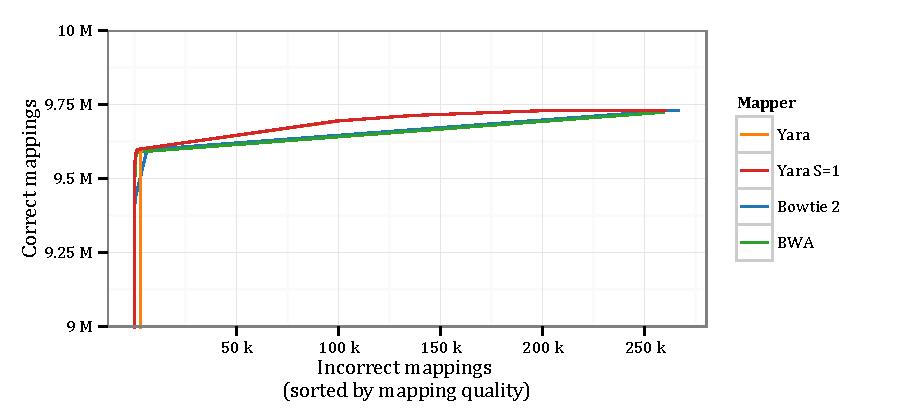
\includegraphics{hiseq_hg19_like_se.accuracy.pdf}
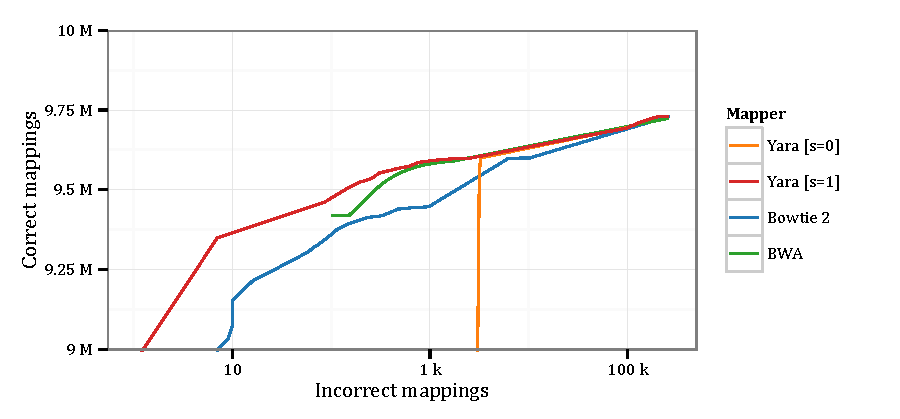
\includegraphics{hiseq_hg19_like_se.accuracy.log.pdf}
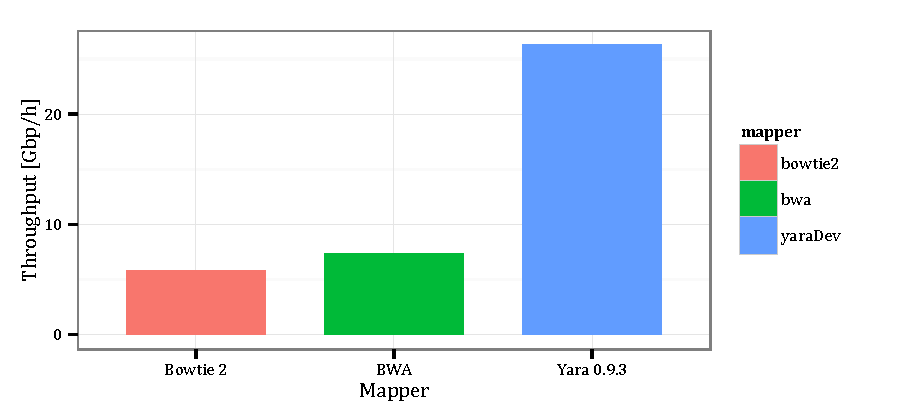
\includegraphics{hiseq_hg19_like_se.default.runtime.pdf}
\end{center}
\end{figure}

%\begin{figure}[t]
%\begin{center}
%\caption[Yara throughput results on simulated single-end data]{Yara throughput results simulated single-end data.}
%\label{fig:yara:throughput-se}
%\end{center}
%\end{figure}

\begin{figure}[t]
\begin{center}
\caption[Yara accuracy results on simulated paired-end data]{Yara accuracy results on simulated paired-end data.}
\label{fig:yara:accuracy-pe}
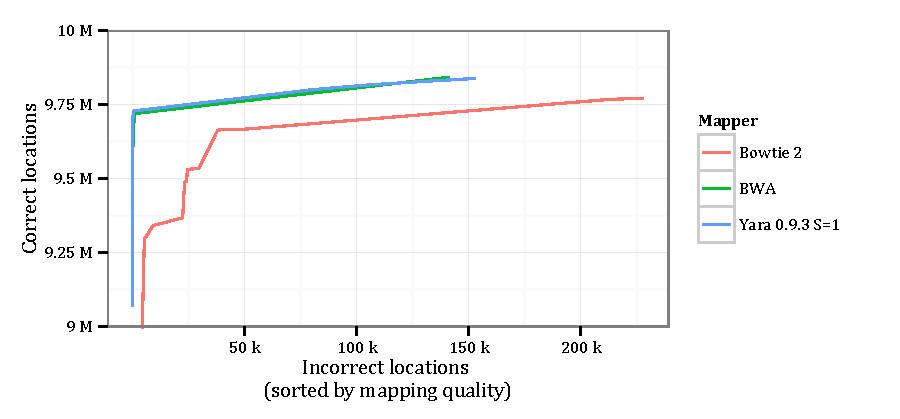
\includegraphics{hiseq_hg19_like_pe.accuracy.pdf}
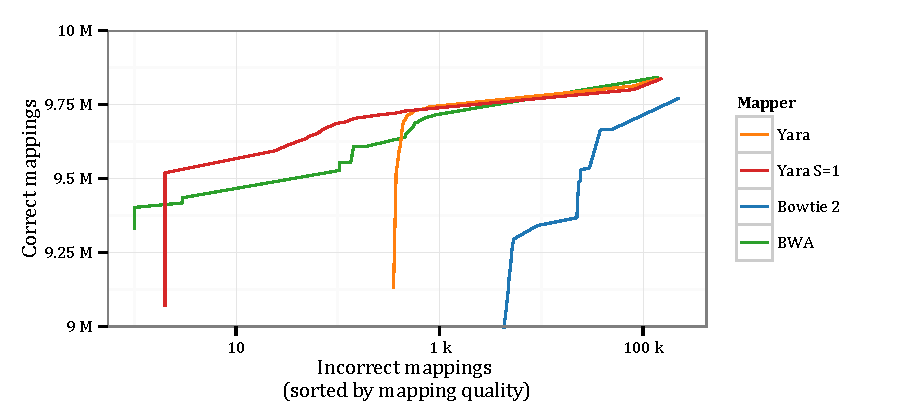
\includegraphics{hiseq_hg19_like_pe.accuracy.log.pdf}
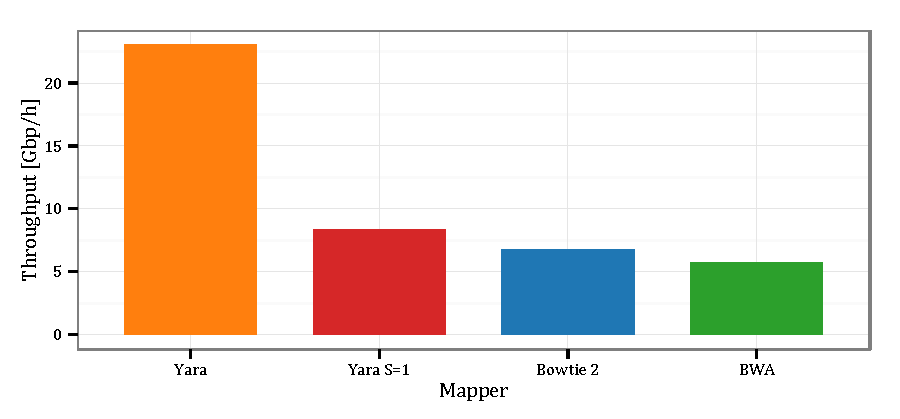
\includegraphics{hiseq_hg19_like_pe.default.runtime.pdf}
\end{center}
\end{figure}

\subsubsection{Single-end reads}
Results are shown in figure~\ref{fig:yara:accuracy-se}.
The ROC curves in the top panel show incorrect locations on a linear scale, in order to highlight unmappable reads.
Conversely, to focus on mappable reads, the ROC curves in the bottom panel show incorrect locations on a logarithmic scale.
From both plots, it is visible that Yara always dominates BWA, which in turn always dominates Bowtie~2.

Comment throughput.

\subsubsection{Paired-end reads}
Results are shown in figure~\ref{fig:yara:accuracy-pe}.
Again, the ROC curves in the top panel show incorrect locations on a linear scale, while, those in the bottom panel are on a logarithmic scale.
Yara still dominates BWA on the most mappable reads; however, compared to single-end reads, BWA on paired-end reads is closer to Yara.
Bowtie~2 shows the worst accuracy. 

Comment throughput.

\subsection{Variant calling on real data}
\label{sec:yara:eval:calling}

% http://www.nature.com/nbt/journal/v32/n3/full/nbt.2835.html

The last experiment uses well-characterized datasets to estimate both true-positive and false-negative rates induced by various mappers within a best-mapping pipeline calling variants on real data.
Each pipeline consists of one best-mapper, whose output is sorted by genomic position using \emph{samtools}, and subsequently given to the the widely used \emph{GATK Unified Genotyper} (UG) \citep{DePristo2012} to call both SNVs and INDELs.
The evaluation consists of comparing the variants called by each pipeline to a set of high-confidence, single-nucleotide variant (SNV) and INDEL calls provided by the \emph{Genome in a Bottle} (GIAB) consortium \citep{Zook2014}.

The GIAB consortium provides a set of calls (NIST v2.18) for the pilot genome NA12878.
Each pipeline has to calls variants from an exome re-sequencing (SRA/ENA id: SRR1611178) of the same NA12878 individual.
This run, produced by the XXX Institute, consists of $2 \times 100\,\text{bp}$ Illumina HiSeq 2000 reads and has a mean coverage of $150$~X.

According to the GIAB guidelines, the evaluation first decomposes complex variants using the tool \emph{vcfallelicprimitives} and subsequently compares called variants to the set of GIAB trusted variants using the tool \emph{UGene XXX}.
This last tool counts the number of correct and incorrect variants, stratifies them by variant quality, and reports their cumulated counts.
The output of the evaluation is plotted as ROC curves.

\begin{figure}[t]
\begin{center}
\caption[SNPs calling accuracy results]{SNVs calling accuracy results.}
\label{fig:yara:calling-snps}
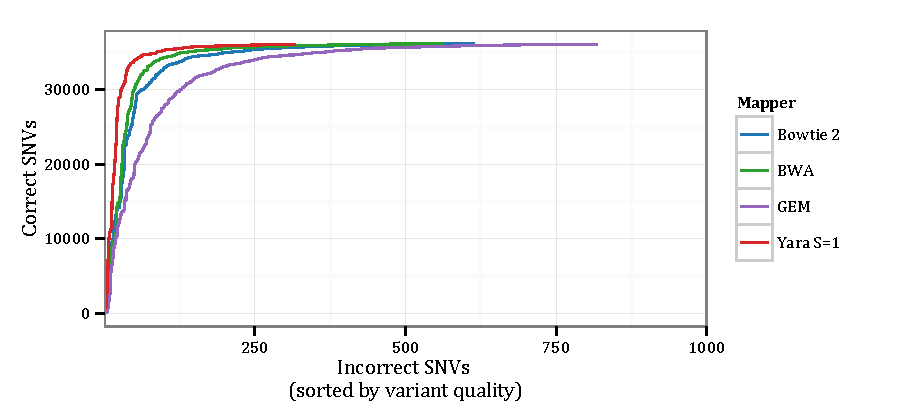
\includegraphics{SRR1611178.snp.pdf}
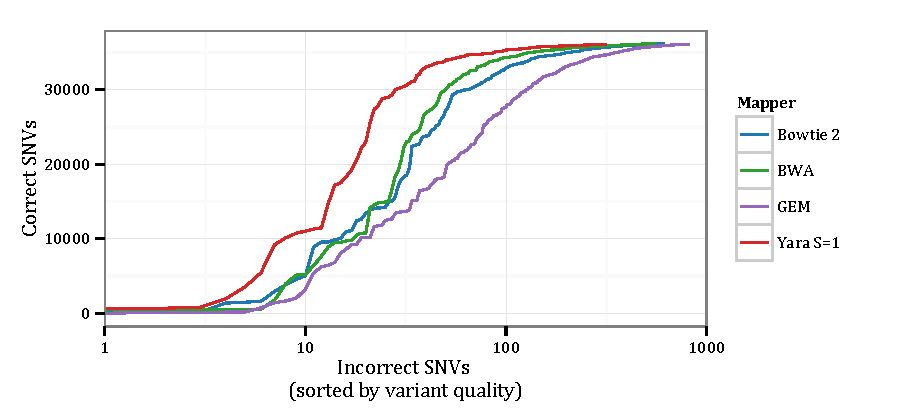
\includegraphics{SRR1611178.snp.log.pdf}
\end{center}
\end{figure}

\begin{figure}[t]
\begin{center}
\caption[INDELs calling accuracy results]{INDELs calling accuracy results.}
\label{fig:yara:calling-indels}
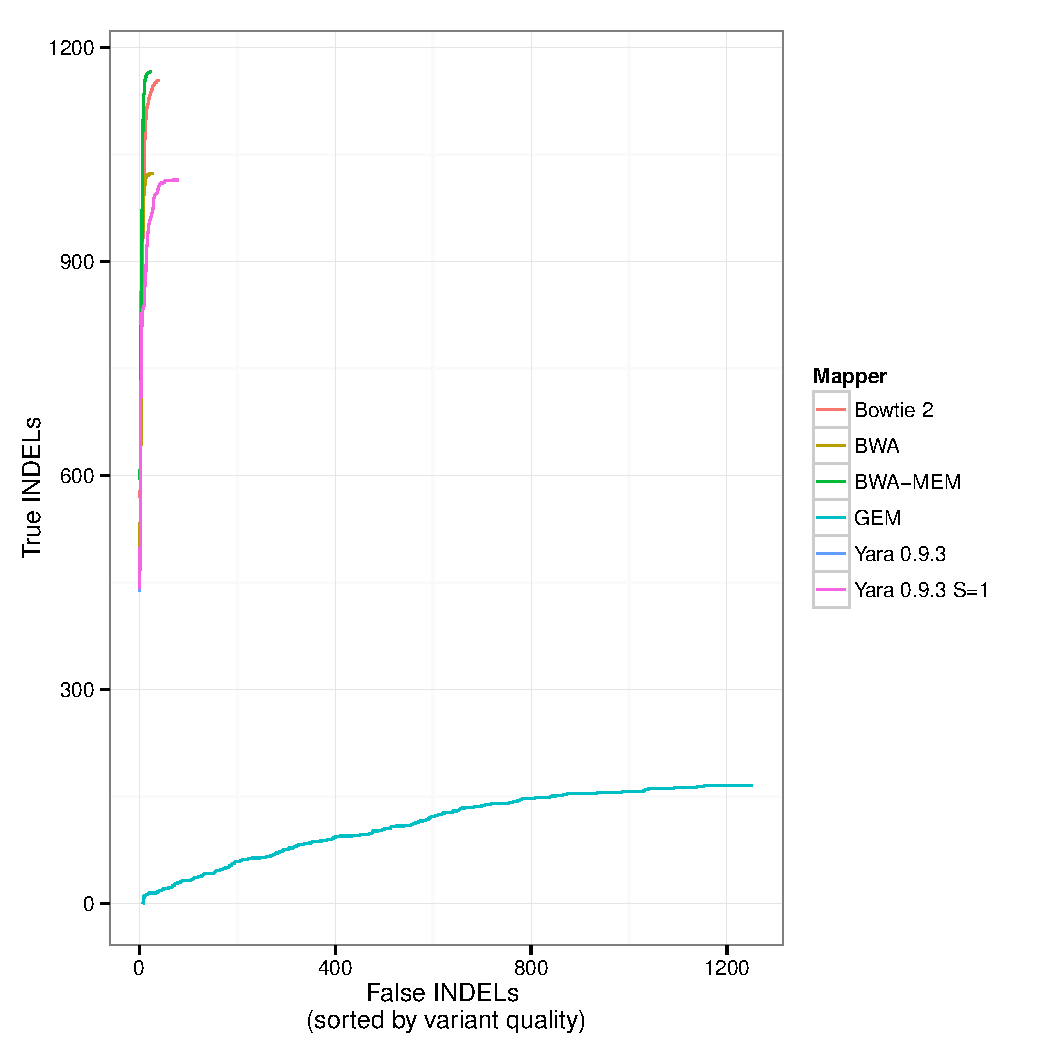
\includegraphics{SRR1611178.indel.pdf}
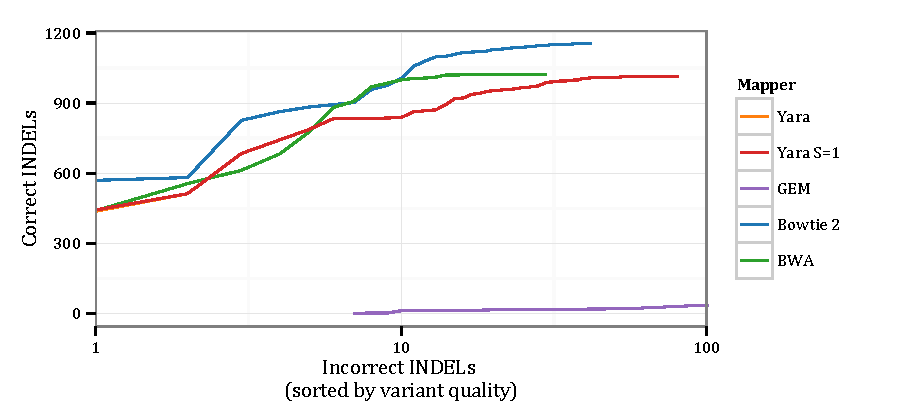
\includegraphics{SRR1611178.indel.log.pdf}
\end{center}
\end{figure}

\begin{figure}[t]
\begin{center}
\caption[Throughput results]{Throughput results.}
\label{fig:yara:throughput}
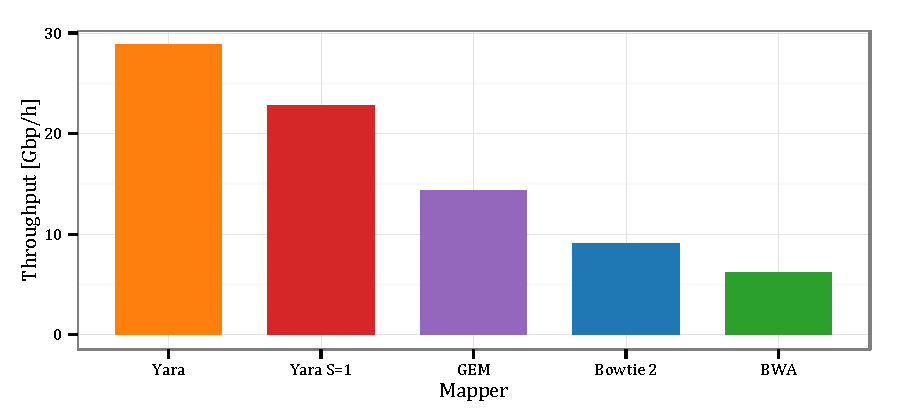
\includegraphics{SRR1611178.default.runtime.pdf}
\end{center}
\end{figure}


\subsubsection{SNVs calling}
Figure~\ref{fig:yara:calling-snps} shows the SNVs calling accuracy results.
The ROC curves in the top panel show incorrect SNVs on a linear scale, in order to low-quality calls.
Conversely, to focus on high-quality calls, the ROC curves in the bottom panel show incorrect SNVs on a logarithmic scale.
From the top curves is evident that Yara induces up to 3 times fewer incorrect SNVs than BWA, while
from the bottom curves is clear that Yara induces a significantly higher number of high-quality calls.
The poor performance of GEM is interesting, as the tool does not annotate mapping locations with qualities.

\subsubsection{INDELs calling}
Figure~\ref{fig:yara:calling-indels} shows the INDELs calling accuracy results.
Again, the ROC curves in the top panel show incorrect INDELs on a linear scale, while, those in the bottom panel are on a logarithmic scale.
Bowtie~2 dominates both BWA and Yara, possibly thanks to the fact that it performs local alignments rather than semi-global alignments.
Yara induces the same number of correct INDEL calls as BWA, although with a higher rate of incorrect calls.

\subsubsection{Throughput}
Comment throughput.


% -----------------------------------------------------------------------------

%\section{Discussion}

%Yara does not consider local alignments and chimeric reads.
